\documentclass[11pt, a4paper]{scrartcl}

% ---- Typography & Layout ----
\usepackage[T1]{fontenc}
\usepackage{lmodern}
\usepackage{microtype}
\usepackage[margin=2.5cm]{geometry}

% ---- Bibliography (arXiv-friendly) ----
\usepackage[numbers,sort&compress]{natbib}

% ---- Math ----
\usepackage{amsmath}
\usepackage{amsthm}
\usepackage{amssymb}
\usepackage{mathtools}

% ---- Custom macros ----
\usepackage{maxicp}

% ---- Lists ----
\usepackage{enumitem}

% ---- Figures ----
\usepackage{graphicx}
\usepackage{subcaption}

% ---- TikZ ----
\usepackage{tikz}
\usepackage{tikz-cd}
\usetikzlibrary{positioning, arrows.meta, shapes.geometric}

\tikzset{
  member/.style={circle, draw=black, fill=white, thick, minimum size=7mm, font=\small},
  possible/.style={circle, draw=gray, fill=gray!15, thick, minimum size=7mm, font=\small},
  required/.style={circle, draw=blue!70, fill=blue!10, thick, minimum size=7mm, font=\small},
  excluded/.style={circle, draw=red!70, fill=red!10, thick, dashed, minimum size=7mm, font=\small},
  successor/.style={->, thick, >=LaTeX},
  insertionDirected/.style={->, dashed, gray, >=LaTeX, bend left=15}
}

% ---- Colors ----
\usepackage{xcolor}

% ---- Algorithms ----
\usepackage[linesnumbered,ruled,noend]{algorithm2e}

% ---- Code listings: listings + tcolorbox (arXiv-friendly) ----
\usepackage{listings}
\usepackage[most]{tcolorbox}
\tcbuselibrary{listings}

% Java syntax highlighting with listings (works on arXiv, no shell-escape)
\definecolor{javakeyword}{RGB}{0,70,160}
\definecolor{javatype}{RGB}{102,14,122}
\definecolor{javastring}{RGB}{163,21,21}
\definecolor{javacomment}{RGB}{0,128,0}

\lstdefinestyle{maxicpjava}{
    language=Java,
    basicstyle=\ttfamily\small,
    keywordstyle=\color{javakeyword}\bfseries,
    keywordstyle=[2]\color{javatype}\bfseries,
    commentstyle=\color{javacomment}\itshape,
    stringstyle=\color{javastring},
    breaklines=true,
    tabsize=3,
    columns=fullflexible,
    keepspaces=true,
    showstringspaces=false,
    morekeywords=[2]{CPIntVar,CPBoolVar,CPSeqVar,CPIntervalVar,CPSolver,DFSearch,SearchStatistics,Objective,ModelDispatcher,IntVar,IntExpression,ConcreteCPModel,StateManager,StateInt,StateMap,DeltaCPIntVar,AbstractConstraint,AbstractCPConstraint}
}

\newtcblisting[auto counter]{codebox}[2][]{%
    listing engine=listings,
    listing options={
        style=maxicpjava
    },
  colback=gray!3,
  colframe=gray!50!black,
  listing only,
  left=3mm, right=3mm, top=2mm, bottom=2mm,
  arc=1mm,
  boxrule=0.5pt,
  title={Listing~\thetcbcounter: #2},
  fonttitle=\small\bfseries,
  #1
}

% ---- Hyperlinks ----
\usepackage{hyperref}

% ---- Theorems ----
\newtheorem{example}{Example}
\newtheorem{theorem}{Theorem}
\newtheorem{definition}{Definition}
\newtheorem{proposition}{Proposition}

% ---- Solver names & shortcuts ----
\newcommand{\ortools}{\textsf{OR-Tools}}
\newcommand{\gecode}{\textsf{Gecode}}
\newcommand{\choco}{\textsf{Choco}}
\newcommand{\optalcp}{\textsf{OptalCP}}
\newcommand{\maxicp}{\textsf{MaxiCP}}
\newcommand{\objectivecp}{\textsf{Objective-CP}}
\newcommand{\minicp}{\textsf{MiniCP}}
\newcommand{\oscar}{\textsf{OscaR}}
\newcommand{\cpoptimizer}{\textsf{CP Optimizer}}
\newcommand{\NB}{N}
\newcommand{\singleDerives}[1]{\underset{\scriptstyle#1}{\longmapsto}}

% ---- Authors ----
\usepackage{authblk}
\usepackage{orcidlink}
\title{\maxicp: A Not So Mini Constraint Programming Solver}
\author[1]{Pierre Schaus\,\orcidlink{0000-0002-3153-8941}}
\author[2]{Guillaume Derval\,\orcidlink{0000-0002-6700-3519}}
\author[3]{Augustin Delecluse\,\orcidlink{0000-0001-6285-6515}\authorcr}
\author[4]{Laurent Michel\,\orcidlink{0000-0001-7230-7130}}
\author[5]{Pascal Van Hentenryck\,\orcidlink{0000-0001-7085-9994}}
\affil[1]{UCLouvain, ICTEAM, Louvain-la-Neuve, Belgium}
\affil[2]{ULi\`ege, Montefiore Institute, Li\`ege, Belgium}
\affil[3]{KU~Leuven, Leuven, Belgium}
\affil[4]{University of Connecticut, Storrs, USA}
\affil[5]{Georgia Institute of Technology, Atlanta, USA}
\date{}

\begin{document}

\maketitle

\begin{abstract}
Constraint Programming (CP) is a powerful paradigm for solving complex combinatorial optimization problems.
This paper presents \maxicp, a modern, high-performance, open-source CP solver designed to bridge the gap between educational simplicity and industrial-grade efficiency.
Building upon \minicp~\cite{Michel2021MiniCP} and incorporating ideas from the \oscar\ solver \cite{oscar}and \objectivecp\ \cite{van2013objective}, \maxicp\ \cite{maxicp_solver} introduces several novelties:
(1) conditional time-interval variables and cumulative functions for scheduling, implemented through the Generalized Cumulative constraint~\cite{Schaus2025GeneralizedCumulative}.
(2) sequence variables' computational domain for routing, supporting insertion-based search heuristics and Large Neighborhood Search~\cite{Schaus2022SeqVar} and
(3) a symbolic modeling layer (\maxicp-Modelling) that treats models as first-class immutable objects, enabling model transformations, reformulations, and parallel resolution strategies~\cite{Derval2023Symbolism};
We provide a detailed description of the solver's architecture, including its state management system based on trailing, its event-driven propagation engine, and its two-layer API design.
Through a series of  models, we show the expressive power of \maxicp.
All source code of \maxicp\ and models are available as an open-source Java library under the MIT license.
\end{abstract}


% ==================================================================================
\section{Introduction}
\label{sec:intro}
% ==================================================================================

Constraint Programming (CP) provides a declarative framework where combinatorial problems are modeled in terms of variables and constraints. The resolution process combines exhaustive search with filtering algorithms (propagators) that prune the search space by removing inconsistent values from variable domains.
The paradigm $\mathit{CP} = \textit{Model} + \textit{Search}$ captures its essence: a user writes a model, and the solver searches for solutions, guided by customizable search heuristics.

CP has been successfully applied to a wide range of industrial applications, from scheduling~\cite{laborie2018ibm} and routing~\cite{kilby2006vehicle} to configuration,
timetabling, and resource allocation.
Commercial solvers such as IBM’s CP Optimizer~\cite{laborie2018ibm} or OptalCP~\cite{optalcp_solver} provides high performance and rich modeling abstractions,
but their proprietary nature restricts access to their internal implementations,
which limits their use in research and education where source code access is often required for experimentation and extension.
Open-source solvers, on the other hand, vary widely in completeness and documentation.
Notable open-source solvers are \choco~\cite{choco}, \gecode~\cite{gecode} and \ortools~\cite{ortools} with a very rich documentation,
that are also high quality solvers that have been maintained over the years.

The architecture of \maxicp\ builds upon \minicp~\cite{Michel2021MiniCP},
which was originally designed as a lightweight, educational solver to illustrate the core principles of constraint programming.
Its elegant and minimalist design offers a near one-to-one correspondence between theoretical CP concepts and their implementation,
making it an excellent pedagogical tool.
However, \minicp\ is not intended for industrial-scale applications.
It lacks several features required for competitive performance such as rich computational domains, efficient search strategies, and its constraint library remains limited.
Additionally, some parts of the implementation are deliberately not fully optimized, as the primary goal is to prioritize code readability and simplicity.

This does not mean that \maxicp\ sacrifices readability—its codebase also remains clear and well-structured.
It incorporates algorithmic ideas from the \oscar\ \cite{oscar} and \objectivecp\ \cite{van2013objective} CP solvers
such as priority-based propagation queues, incremental constraint computations based on advanced mechanisms such as delta changes of the domains \cite{sparsets2013domain}.
It also includes novel functionalities such as insertion-based sequence variables \cite{delecluse2022sequence,Schaus2022SeqVar,Schaus2022SeqVar},
some of them highly inspired from commercial solvers such as conditional task intervals \cite{LaborieR08,LaborieRSV09}.
\maxicp\ also proposes some efficient black-box search strategies such as Conflict Ordering Search \cite{conflictOrderingSearch} or Failure Directed Search \cite{failureDirectedSearch}.
The result is a solver that is simultaneously well-suited for education, research, and practical deployment.

Like its predecessor \minicp, \maxicp\ is implemented in Java\footnote{Java offers an excellent trade-off between ease of development, code stability, ease of use, and execution speed.
Its strong type system, automatic memory management, and mature tooling ecosystem
make it well suited for building complex combinatorial solvers that remain maintainable over time.
Moreover, recent advances in the Java ecosystem, such as ahead-of-time compilation to native code (e.g., via GraalVM), further improve performance and deployment flexibility.}
similarly to other successful CP solvers (e.g. \choco~\cite{choco}, or ACE solver~\cite{ace}).

\paragraph{Scope of this document.}
This document is not intended as an introduction to Constraint Programming.
Readers seeking a conceptual overview of CP---including domains, propagation, and search---are referred to the \minicp\ paper~\cite{Michel2021MiniCP} and related literature (e.g. \cite{lecoutre2013constraint}).
Instead, this document illustrates the main functionalities of \maxicp to model and solve combinatorial optimization problems.

More specifically, the document:
\begin{itemize}[leftmargin=*]
    \item presents the main modeling and solving capabilities of \maxicp, illustrated through representative code examples;
    \item demonstrates how common problem classes---including combinatorial optimization, scheduling, and vehicle routing---can be expressed using appropriate variables, constraints, and search strategies;
    \item describes the two-level design of the API, distinguishing between the low-level engine interface and the higher-level symbolic modeling layer.
\end{itemize}

\noindent
The primary functionalities of \maxicp\ discussed in this document are:

\begin{itemize}[leftmargin=*]

    \item \textbf{Basic Functionalities}:
    This includes the state-management and the trail, implementing a custom search, implementing a constraint, and solving a problem with Large Neighborhood Search (LNS) \cite{shaw1998using}.

    \item \textbf{Advanced Scheduling with Conditional Time Intervals}:
    Full support for conditional time-interval variables and cumulative function expressions, as introduced in~\cite{LaborieRSV09} and implemented through the Generalized Cumulative constraint~\cite{Schaus2025GeneralizedCumulative}. This enables the natural modeling of optional tasks, alternative resources, and producer-consumer scheduling problems.

    \item \textbf{Sequence Variables (\texttt{SeqVar})}:
    A dedicated computational domain for routing and sequencing problems~\cite{Schaus2022SeqVar}. Sequence variables represent partial paths through node insertions rather than successor arrays, natively supporting optional visits, insertion-based search heuristics, and Large Neighborhood Search. Dedicated global constraints such as \texttt{distance}, \texttt{transitionTimes}, and \texttt{cumulative} are provided for vehicle routing.


    \item \textbf{Symbolic Modeling (\maxicp-Modelling)}:
    A modeling layer that treats models as immutable symbolic linked lists of constraints~\cite{Derval2023Symbolism}. 
    This design enables model transformations and reformulations, the creation of sub-problems and neighborhoods for Large Neighborhood Search, 
    and embarrassingly parallel search where multiple solver instances work on the same immutable model.

\end{itemize}

The remainder of this paper is structured as follows.
Section~\ref{sec:architecture} gives an overview of the architecture, introduces the package organization, and presents the two-layer API (raw and symbolic) through a side-by-side comparison on the N-Queens problem.
From Section~\ref{sec:state} onward, we adopt a bottom-up presentation, starting with the implementation layer:
Section~\ref{sec:state} covers state management and trailing,
Section~\ref{sec:propagation} details the propagation engine,
Section~\ref{sec:search} covers the search framework including Large Neighborhood Search (LNS) \cite{shaw1998using} and Variable Objective Large Neighborhood Search (VOLNS) \cite{volns}.
We then turn to advanced variable domains:
Section~\ref{sec:scheduling} covers conditional time-interval variables and scheduling,
Section~\ref{sec:seqvar} presents sequence variables for routing,
We finish by introducing the symbolic modeling in Section~\ref{sec:symbolism} and its support for model transformations, reformulations, and parallel search.
Section~\ref{sec:conclusion} concludes.


% ==================================================================================
\section{Architecture Overview}
\label{sec:architecture}
% ==================================================================================

\maxicp\ is implemented in Java (version 17+) and consists of approximately 40\,000 lines of code.
Its architecture is organized into several coherent packages:

\begin{description}[leftmargin=0pt, labelwidth=0pt, itemindent=!]
    \item[\texttt{org.maxicp.state}] provides the state management primitives and data-structures used for backtracking and the \emph{trailing} default implementation.

    \item[\texttt{org.maxicp.cp.engine.core}] contains the core CP engine: the solver (\texttt{MaxiCP}), variable implementations (\texttt{CPIntVar}, \texttt{CPBoolVar}, \texttt{CPSeqVar}, \texttt{CPIntervalVar}), domains, and the priority-based propagation queue.

    \item[\texttt{org.maxicp.cp.engine.constraints}] contains the constraint implementations, organized into sub-packages for some specific computation domains.

    \item[\texttt{org.maxicp.modeling}] provides the symbolic modeling layer, including symbolic variables (\texttt{IntVar}, \texttt{SeqVar}, \texttt{IntervalVar}), the \texttt{Factory} with constraint creation methods, and the symbolic model representation.

    \item[\texttt{org.maxicp.cp.modeling}] bridges the symbolic modeling layer and the concrete CP layers. The \texttt{ConcreteCPModel} class instantiates symbolic constraints into the CP engine.

    \item[\texttt{org.maxicp.search}] implements search strategies, including depth-first search (\texttt{DFSearch}), concurrent search (\texttt{ConcurrentDFSearch}), best-first search (\texttt{BestFirstSearch}), and a rich library of variable and value selection heuristics (\texttt{Searches}).
\end{description}

\subsection{Two Levels of Modeling: Raw and Symbolic}
\label{sec:two-layer-overview}

A distinguishing feature of \maxicp\ is that it offers \emph{two} ways to model and solve problems:

\begin{enumerate}
    \item \textbf{The raw (engine-level) API.}
    The user creates a \texttt{CPSolver} instance and works directly with concrete variable objects (\texttt{CPIntVar}, \texttt{CPSeqVar}, \texttt{CPIntervalVar}).
    Constraints are posted on the solver via \texttt{cp.post(...)}.
    Branching closures modify the solver state by posting equality/dis\-equality constraints.
    This API gives maximal control over the engine and is the natural choice when implementing custom constraints, propagators, or search heuristics.
    It mirrors the API of \minicp, so users familiar with \minicp\ will feel immediately at home.

    \item \textbf{The symbolic (modeling-level) API.}
    The user creates a \texttt{ModelDispatcher} and works with symbolic variable objects (\texttt{IntVar}, \texttt{SeqVar}, \texttt{IntervalVar}).
    Constraints are added via \texttt{model.add(...)}.
    The model is an immutable linked list; adding a constraint returns a new model node, leaving the original unchanged.
    The model must be \emph{concretized} into a solver engine before it can be solved.
    This indirection enables model transformations, LNS neighborhoods as model branches, and embarrassingly parallel search.
    The symbolic layer is described in detail in Section~\ref{sec:symbolism}.
\end{enumerate}

The two APIs are remarkably similar in surface syntax.
To illustrate this, Listings~\ref{lst:nqueens-raw} and~\ref{lst:nqueens-modeling} show the NQueens problem implemented in each style.

\begin{codebox}[label={lst:nqueens-raw}]{N-Queens with the raw API (\texttt{CPSolver})}
int n = 8;
CPSolver cp = CPFactory.makeSolver();
CPIntVar[] q  = CPFactory.makeIntVarArray(cp, n, n);
CPIntVar[] qL = CPFactory.makeIntVarArray(n, i -> minus(q[i], i));
CPIntVar[] qR = CPFactory.makeIntVarArray(n, i -> plus(q[i], i));

cp.post(allDifferent(q));
cp.post(allDifferent(qL));
cp.post(allDifferent(qR));

DFSearch search = CPFactory.makeDfs(cp, () -> {
    CPIntVar qs = selectMin(q,
            qi -> qi.size() > 1,
            qi -> qi.size());
    if (qs == null) return EMPTY;
    int v = qs.min();
    return branch(
        () -> cp.post(eq(qs, v)),
        () -> cp.post(neq(qs, v)));
});

search.onSolution(() ->
    System.out.println(Arrays.toString(q)));
SearchStatistics stats = search.solve();
\end{codebox}

\begin{codebox}[label={lst:nqueens-modeling}]{N-Queens with the symbolic API (\texttt{ModelDispatcher})}
int n = 12;
ModelDispatcher model = makeModelDispatcher();
IntVar[] q  = model.intVarArray(n, n);
IntExpression[] qL = model.intVarArray(n, i -> q[i].plus(i));
IntExpression[] qR = model.intVarArray(n, i -> q[i].minus(i));

model.add(allDifferent(q));
model.add(allDifferent(qL));
model.add(allDifferent(qR));

Supplier<Runnable[]> branching = () -> {
    IntExpression qs = selectMin(q,
            qi -> qi.size() > 1,
            qi -> qi.size());
    if (qs == null) return EMPTY;
    int v = qs.min();
    return branch(
        () -> model.add(eq(qs, v)),
        () -> model.add(neq(qs, v)));
};

ConcreteCPModel cp = model.cpInstantiate();
DFSearch dfs = cp.dfSearch(branching);
dfs.onSolution(() ->
    System.out.println(Arrays.toString(q)));
SearchStatistics stats = dfs.solve();
\end{codebox}

Both APIs share the same search infrastructure (\texttt{DFSearch}, \texttt{SearchStatistics}, \texttt{Searches}), the same heuristics (\texttt{firstFailBinary}, \texttt{setTimes}, etc.), and the same constraint library.
The branching function in the NQueens examples defines a custom search strategy
where the solver selects the variable with the smallest domain (first-fail heuristic)
and branches by assigning its minimum value or removing it.
While writing custom branching closures provides complete control over the search,
as detailed in Section~\ref{sec:search}, \maxicp\ also provides a variety of
pre-built heuristics and combinators that simplify search definition.
In the following sections we adopt a bottom-up presentation, starting from the implementation of the (raw) layer main objects: state management, propagation, and search.
The symbolic modeling layer is covered in depth in Section~\ref{sec:symbolism}.

% ==================================================================================
\section{State Management}
\label{sec:state}
% ==================================================================================

CP solvers must efficiently save and restore states during search, which is inherently organized as a depth-first search (DFS).
In DFS-based constraint programming, the solver explores a decision tree by making a branching decision, recursively continuing the search, and backtracking when a failure or dead-end is reached.
This execution model requires a mechanism to restore a previous consistent state before exploring an alternative branch.
\maxicp\ is a \emph{trail-based} solver: rather than saving the entire state at each choice point, it relies on a stack-based memory management scheme called the \emph{trail}.
We refer to \cite{Michel2021MiniCP} for a comprehensive introduction to trailing and its implementation in CP solvers.
Very briefly, the trail records only the incremental changes that occur during propagation and search.
This makes it possible to efficiently undo modifications when backtracking in the DFS tree.
The trail mechanism is available through the \texttt{StateManager} interface that exposes the following key operations:

\begin{codebox}{StateManager interface}
public interface StateManager {
    void saveState();       // Push a new save point
    void restoreState();    // Restore to last save point
    int getLevel();         // Current depth in the tree

    StateInt makeStateInt(int initValue);
    <T> State<T> makeStateRef(T initValue);
    <K,V> StateMap<K,V> makeStateMap();
}
\end{codebox}

All stateful components of the solver---variable domains, propagation queues, the depth first search and even the symbolic model reference---are built on top of these primitives.
For instance, the domain of a \texttt{CPIntVar} is backed by \texttt{StateInt} (i.e. reversible integers) for its minimum and maximum bounds,
and by a reversible sparse set for the set of values in the domain \cite{sparsets2013domain,Michel2021MiniCP}.

\paragraph{Usage Example.}
Listing~\ref{lst:trailing-example} illustrates the use of trailing:

\begin{codebox}[label={lst:trailing-example}]{Trailing example in MaxiCP}
StateManager sm = new Trailer();
StateInt counter = sm.makeStateInt(0);

sm.saveState();           // Level 0 -> Level 1
counter.setValue(10);     // Trail records: (counter, 0)

sm.saveState();           // Level 1 -> Level 2
counter.setValue(42);     // Trail records: (counter, 10)

sm.restoreState();        // Level 2 -> Level 1, counter = 10
sm.restoreState();        // Level 1 -> Level 0, counter = 0
\end{codebox}

The trailing mechanism is implemented in the \texttt{Trailer} class.
Conceptually, every time the solver descends in the search tree, it creates a new decision level by calling the \texttt{saveState()} method,
which pushes a new save point onto the trail stack.
Any modification performed at that level is recorded in the trail so that it can be undone when the solver returns to a previous level on backtrack.

% ==================================================================================
\section{Propagation Engine}
\label{sec:propagation}
% ==================================================================================

The propagation engine is the heart of any CP solver. In \maxicp, it is implemented in the \texttt{MaxiCP} class and follows a priority-based fixed-point algorithm.

\subsection{Priority-Based Scheduling}

Constraints in \maxicp\ implement the \texttt{CPConstraint} interface, which defines a \texttt{propagate()} method and a \texttt{priority()} method. When a variable domain changes, the constraints that are subscribed to that event are \emph{scheduled} for propagation. The engine processes constraints from a priority queue, ensuring that lightweight, fast-propagating constraints (e.g., unary constraints, equality) are executed before expensive global constraints (e.g., \texttt{AllDifferent}, \texttt{Cumulative}).

\begin{codebox}{The fixed-point propagation loop in MaxiCP}
public void fixPoint() {
    notifyFixPoint();
    while (!propagationQueue.isEmpty()) {
        CPConstraint c = propagationQueue.poll();
        c.setScheduled(false);
        if (c.isActive())
            c.propagate();
    }
}

public void schedule(CPConstraint c) {
    if (c.isActive() && !c.isScheduled()) {
        c.setScheduled(true);
        propagationQueue.add(c, c.priority());
    }
}
\end{codebox}

If a constraint's propagation triggers an \texttt{InconsistencyException}, the queue is cleared and the exception propagates up to the search layer, which handles backtracking.

\subsection{Event-Driven Constraint Activation}

Constraints register themselves to specific domain events. When a variable's domain is modified, only the relevant constraints are re-scheduled. The available events depend on the variable type:

\begin{itemize}
    \item \textbf{Integer variables (\texttt{CPIntVar}):}
    \begin{itemize}
        \item \texttt{propagateOnFix}: triggered when the variable is assigned a single value.
        \item \texttt{propagateOnBoundChange}: triggered when the minimum or maximum of the domain changes.
        \item \texttt{propagateOnDomainChange}: triggered when any value is removed from the domain.
    \end{itemize}
    \item \textbf{Interval variables (\texttt{CPIntervalVar}):}
    \begin{itemize}
        \item \texttt{propagateOnChange}: triggered when any attribute of the interval (start, end, length, presence) changes.
        \item \texttt{propagateOnFix}: triggered when the interval is fully fixed.
    \end{itemize}

    \item \textbf{Sequence variables (\texttt{CPSeqVar}):}
    \begin{itemize}
        \item \texttt{propagateOnInsert}: triggered when a node is inserted into the partial sequence.
        \item \texttt{propagateOnExclude}: triggered when a node is excluded from the sequence.
        \item \texttt{propagateOnRequire}: triggered when a node becomes required.
    \end{itemize}


\end{itemize}

This fine-grained event system avoids unnecessary re-propagation and is critical for the solver's performance.
Notice that registering a constraint to an event is a reversible operation:
it becomes part of the current search state and will automatically be undone upon backtracking thanks to the trail-based state management.

\subsection{Posting Constraints}

Constraints are posted to the solver using \texttt{cp.post(constraint)}.
Due to the reversibility of constraint registration, posting a constraint is also a reversible operation:
it becomes part of the current search state and will automatically be undone upon backtracking thanks to the trail-based state management.
This property is important in a depth-first search setting, where alternative branches are explored by temporarily extending the current state rather than copying it.

This method invokes the constraint's \texttt{post()} method, which typically:
\begin{enumerate}
    \item Registers the constraint to the relevant variable events.
    \item Performs an initial propagation.
\end{enumerate}

By default, posting a constraint immediately triggers a full fixed-point computation,
ensuring that all propagation consequences of the new constraint are fully enforced before search continues.
This behavior is precisely why constraint posting is well-suited for branching:
search decisions can be implemented by posting constraints that define each alternative branch,
letting propagation automatically explore their consequences.

This propagation step can be deferred by passing \texttt{false} as a second argument, i.e., \texttt{cp.post(constraint, false)}.
The fix-point can then be explicitly triggered later by calling \texttt{cp.fixPoint()}.

When posting a constraint, the constraint can fail immediately if it detects an inconsistency (e.g., an empty domain).
In this case, an \texttt{InconsistencyException} is thrown, which is caught by the search engine to trigger backtracking.

\subsection{Implementing a Custom Constraint}

Implementing a custom constraint in \maxicp\ involves extending the \texttt{AbstractConstraint} class and
implementing the \texttt{post()} and \texttt{propagate()} methods.
Listing~\ref{lst:custom-constraint} shows the implementation of a $x \leq y$ constraint.

\begin{codebox}[label={lst:custom-constraint}]{Implementation of the LessOrEqual constraint}
public class LessOrEqual extends AbstractConstraint {
    private final CPIntVar x, y;

    public LessOrEqual(CPIntVar x, CPIntVar y) {
        super(x.getSolver());
        this.x = x; this.y = y;
    }

    @Override
    public void post() {
        x.propagateOnBoundChange(this);
        y.propagateOnBoundChange(this);
        propagate();
    }

    @Override
    public void propagate() {
        x.removeAbove(y.max());
        y.removeBelow(x.min());
    }
}
\end{codebox}

The \texttt{post()} method is responsible for registering the constraint to variable events.
In this case, the constraint is re-scheduled whenever the upper bound of $x$ or the lower bound of $y$ changes.
The \texttt{propagate()} method then prunes the domains.
Whenever a domain becomes empty, through the call to \texttt{removeAbove} or \texttt{removeBelow},
an \texttt{InconsistencyException} is thrown, which signals the search engine to backtrack.
For some constraint, it may be necessary to explicitly throw an \texttt{InconsistencyException} when a failure is detected.

\subsection{Implementing a Custom Constraint with Delta}

A more efficient way to implement propagators is to take advantage of \textit{delta events},
which allow the constraint to react only to changes in variable domains rather
than re-scanning full domains at each propagation.
This is explained in \cite{sparsets2013domain}.

Listing~\ref{lst:element-delta-1} and \ref{lst:element-delta-2} show a possible implementation of a $\texttt{Element}$ constraint,
which enforces $z = t[y]$ using delta-based incremental propagation.

The constraint maintains two-directional consistency between $y$ and $z$:
\begin{itemize}
    \item A value $v \in \mathrm{dom}(y)$ is \emph{supported} if and only if $t[v] \in \mathrm{dom}(z)$.
          When a value is removed from $\mathrm{dom}(z)$, every index $v$ in $\mathrm{dom}(y)$ with $t[v] = v$ loses its support and must be removed.
    \item A value $w \in \mathrm{dom}(z)$ is \emph{supported} if and only as there exists at least one index $v \in \mathrm{dom}(y)$ such that $t[v] = w$.
          When that count drops to zero, $w$ can no longer be achieved and must be removed from $\mathrm{dom}(z)$.
\end{itemize}

The key data structure is \texttt{supportCounter},
an array of \emph{reversible integers} (i.e.\ \texttt{StateInt} objects backed by the trail).
Its size equals the initial size of $\mathrm{dom}(z)$, and it is indexed by \texttt{v - offZ},
where \texttt{offZ = z.min()} is the offset recorded at posting time.

\[
  \texttt{supportCounter}[w - \texttt{offZ}]
  \;=\;
  \bigl|\{\, v \in \mathrm{dom}(y) \mid t[v] = w \,\}\bigr|
\]

In words, \texttt{supportCounter[w - offZ]} counts the number of indices currently in $\mathrm{dom}(y)$ that map to value $w$ through the array $t$.
This count is computed once during \texttt{post()} and maintained incrementally during \texttt{propagate()}:

\begin{itemize}
    \item When a value $v$ is removed from $\mathrm{dom}(y)$ (detected via \texttt{yDelta}), the counter for $t[v]$ is \emph{decremented}.
          If it reaches $0$, no index in $\mathrm{dom}(y)$ maps to $t[v]$ any more, so $t[v]$ is removed from $\mathrm{dom}(z)$.
    \item When a value $w$ is removed from $\mathrm{dom}(z)$ (detected via \texttt{zDelta}), every index $v \in \mathrm{dom}(y)$ with $t[v] = w$ is removed from $\mathrm{dom}(y)$.
          Note that these removals will in turn trigger further decrements of the affected counters, but since $w$ is already gone from $\mathrm{dom}(z)$, those counters reaching $0$ require no further action.
\end{itemize}

Because \texttt{supportCounter} elements are \texttt{StateInt} objects, their values are automatically restored upon backtracking,
keeping the counters consistent with the current search state at every node of the search tree.

The objects \texttt{yDelta} and \texttt{zDelta} are created by \texttt{y.delta(this)} and \texttt{z.delta(this)} respectively.
A delta tracks, for the constraint which values have been removed from the variable's domain \emph{since the last time this constraint was propagated}.
Calling \texttt{yDelta.fillArray(yValues)} fills the array with those recently removed values and returns their count.
This avoids iterating over the entire remaining domain and is the key mechanism that makes the propagator incremental.

\begin{codebox}[label={lst:element-delta-1}]{Delta-based implementation of Element (part 1)}
public class Element extends AbstractCPConstraint {

    private final int[] t;
    private final CPIntVar y, z;
    private DeltaCPIntVar yDelta, zDelta;
    private int[] yValues, zValues;
    private int offZ;
    private StateInt[] supportCounter;

    public Element(int[] array, CPIntVar y, CPIntVar z) {
        super(y.getSolver());
        this.t = array;
        this.y = y;
        this.z = z;
    }

    @Override
    public void post() {
        y.removeBelow(0);
        y.removeAbove(t.length - 1);
        y.propagateOnDomainChange(this);
        yDelta = y.delta(this);
        yValues = new int[y.size()];

        z.removeBelow(Arrays.stream(t).min().getAsInt());
        z.removeAbove(Arrays.stream(t).max().getAsInt());
        z.propagateOnDomainChange(this);
        zDelta = z.delta(this);
        zValues = new int[z.size()];

        int sizeY = y.fillArray(yValues);
        for (int i = 0; i < sizeY; i++) {
            int v = yValues[i];
            if (!z.contains(t[v])) {
                y.remove(v);
            }
        }
        supportCounter = new StateInt[z.size()];
        offZ = z.min();
        for (int i = 0; i < z.size(); i++) {
            supportCounter[i] =
            getSolver().getStateManager().makeStateInt(0);
        }
        for (int i = 0; i < t.length; i++) {
            if (y.contains(i)) {
                supportCounter[t[i] - offZ].increment();
            }
        }
        int sizeZ = z.fillArray(zValues);
        for (int i = 0; i < sizeZ; i++) {
            int v = zValues[i];
            if (supportCounter[v - offZ].value() == 0) {
                z.remove(v);
            }
        }
        propagate();
    }
}
\end{codebox}

\begin{codebox}[label={lst:element-delta-2}]{Delta-based implementation of Element (part 2)}
@Override
public void propagate() {

    if (zDelta.size() > 0) {
        int size = zDelta.fillArray(zValues);
        for (int i = 0; i < size; i++) {
            int v = zValues[i];

            int sizeY = y.fillArray(yValues);
            for (int j = 0; j < sizeY; j++) {
                int yv = yValues[j];
                if (t[yv] == v) {
                    y.remove(yv);
                }
            }
        }
    }

    if (yDelta.size() > 0) {
        int size = yDelta.fillArray(yValues);
        for (int i = 0; i < size; i++) {
            int v = yValues[i];

            StateInt counter = supportCounter[t[v] - offZ];
            if (counter.decrement() == 0) {
                z.remove(t[v]);
            }
        }
    }
}
\end{codebox}

\subsection{Global Constraints in \maxicp\ }

This subsection lists some important global constraints available in \maxicp,
with their semantics and references on their filtering algorithms.

\paragraph{Table constraint (\texttt{TableCT}).}
Given variables $x = \langle x_1,\ldots,x_n\rangle$ and a table
$T \subseteq \mathbb{Z}^n$, the constraint enforces that the assignment of $x$
matches one row of $T$:
\[
\exists r \in T:\; \forall j \in \{1,\ldots,n\},\; x_j = r_j.
\]
This is the classical extensional (in-extension) constraint.
\maxicp\ relies the compact-table filtering~\cite{demeulenaere2016compact}.

\paragraph{Bin packing constraint (\texttt{BinPacking}).}
Given item-to-bin variables $x_i$, item weights $w_i$, and bin-load variables
$\mathit{load}_b$, the constraint enforces exact bin loads:
\[
\forall b:\; \mathit{load}_b = \sum_{i \mid x_i = b} w_i.
\]
The filtering of relies on~\cite{shaw2004constraint,schaus2009solving,derval2018improved}.

\paragraph{Global cardinality constraint (GCC).}
For value set $V$ and occurrence bounds, GCC constrains the number of
variables taking each value. With upper bounds only (as in
\texttt{CostCardinalityMaxDC} without costs), semantics is:
\[
\forall v \in V:\; \left|\{i \mid x_i = v\}\right| \le U_v.
\]
The arc-consistent filtering is due to R\'egin~\cite{regin1996generalized}
but \maxicp\ relies on the algorithm of~\cite{schmied2025efficient}.

\paragraph{Soft cardinality constraint (\texttt{SoftCardinalityDC}).}
For values $v$ with lower/upper bounds $L_v, U_v$, let
$c_v = \left|\{i \mid x_i = v\}\right|$. The violation per value is
\[
\mathrm{viol}(v) = \max(0, L_v - c_v, c_v - U_v),
\]
and the global violation variable is constrained by
\[
\mathit{viol} = \sum_v \mathrm{viol}(v).
\]
This constraint was introduced in \cite{van2006global} 
but the \maxicp\ filtering relies on the one of ~\cite{schaus2010revisiting,zanarini2006improved}.

\paragraph{Cardinality with costs (\texttt{CostCardinalityMaxDC}).}
With assignment costs $\mathit{cost}_{i,v}$ and budget variable $H$, the
constraint combines (upper-bounded) cardinality and a global cost limit:
\[
\forall v:\; \left|\{i \mid x_i = v\}\right| \le U_v,
\qquad
\sum_i \mathit{cost}_{i,x_i} \le H.
\]
The filtering algorithms for GCC with costs implemented in \maxicp\ is the one of~\cite{schmied2025efficient}.

% ==================================================================================
\section{Search}
\label{sec:search}
% ==================================================================================

\maxicp\ provides a flexible, compositional search framework. The core search engine is a depth-first search with branch-and-bound for optimization.

\subsection{Depth-First Search with Closures}

Following the design of \minicp~\cite{Michel2021MiniCP},
the search in \maxicp\ is defined by a \emph{branching function}:
a supplier of an array of closures (the \texttt{Runnable} functional interface in Java), one for each child branch.
When the array is empty, the current node is considered as a solution.
Listing~\ref{lst:branching} illustrates this concept on the N-Queens problem:

\begin{codebox}[label={lst:branching}]{Branching as a supplier of closures (raw API)}
DFSearch search = makeDfs(cp, () -> {
    CPIntVar qs = selectMin(q, // first-fail: select variable
        qi -> qi.size() > 1, //   that is not fixed
        qi -> qi.size()); //   with smallest domain
    if (qs == null) return EMPTY; // all fixed -> solution
    int v = qs.min();
    return branch(
        () -> cp.post(eq(qs, v)), // left: assign v
        () -> cp.post(neq(qs, v)) // right: remove v
    );
});
\end{codebox}

The \texttt{branch} method returns an array of runnables.
The \texttt{selectMin} utility selects the variable with the smallest domain among unfixed variables, implementing the well-known \emph{first-fail} heuristic.
Each branch closure calls \texttt{cp.post()} to add a constraint.
The posting of the constraint is thus not immediately executed when the branching function is called,
but rather deferred until the corresponding branch is explored in the search tree.
As described in Section~\ref{sec:propagation}, \texttt{post} registers the constraint and triggers a full fix-point computation,
propagating all consequences of the branching decision.
If the fix-point detects an inconsistency (an empty domain), an \texttt{InconsistencyException} is thrown and the search backtracks.

\subsection{Built-In Heuristics: Variable and Value Selectors}

Writing a branching closure from scratch, as in Listing~\ref{lst:branching}, gives full control but is verbose.
The \texttt{Searches} class offers a compositional alternative by separating two orthogonal concerns:
\begin{enumerate}
    \item A \emph{variable selector} (\texttt{Supplier<IntExpression>}): returns the next unfixed variable to branch on, or \texttt{null} when all variables are fixed.
    \item A \emph{value selector} (\texttt{Function<IntExpression, Integer>}): given the selected variable, returns the value to try first.
\end{enumerate}

\noindent
These selectors are combined by the factory methods \texttt{heuristicBinary} and \texttt{heuristicNary} to produce complete branching strategies, as illustrated next on the N-Queens problem.

\paragraph{Binary branching.}
\texttt{heuristicBinary(varSel)} produces a binary branching: at each node, the variable selector picks a variable~$x$; the left branch assigns $x = \min(\text{dom}(x))$ and the right branch removes that value ($x \neq \min(\text{dom}(x))$).
An overload \texttt{heuristicBinary(varSel, valSel)} lets the user supply a custom value selector instead of the default minimum.
Listing~\ref{lst:nqueens-heuristic} shows three equivalent ways to write a first-fail search for NQueens.

\begin{codebox}[label={lst:nqueens-heuristic}]{N-Queens: three ways to express first-fail binary search}
// (a) most concise: built-in convenience method
DFSearch s1 = makeDfs(cp, firstFailBinary(q));

// (b) explicit variable selector, default value (min)
DFSearch s2 = makeDfs(cp,
    heuristicBinary(minDomVariableSelector(q)));

// (c) explicit variable and value selectors
DFSearch s3 = makeDfs(cp,
    heuristicBinary(minDomVariableSelector(q),
                    x -> x.min())); // value = min of domain
\end{codebox}

\noindent
All three produce the same search tree.
Variant~(c) is the most flexible: the value selector can be replaced by any function, e.g.\ \texttt{x -> (x.min() + x.max()) / 2} to branch on the domain midpoint.

\paragraph{N-ary branching.}
\texttt{heuristicNary(varSel)} creates one child branch per value in the domain (in increasing order).
An overload accepts a value heuristic $h : \mathbb{Z} \to \mathbb{Z}$ and sorts the domain values by increasing $h(v)$ before creating the branches.

\begin{codebox}[label={lst:nqueens-nary}]{N-Queens: n-ary branching with custom value ordering}
// n-ary, values tried in increasing order
DFSearch s4 = makeDfs(cp,
    heuristicNary(minDomVariableSelector(q)));

// n-ary: values closer to n/2 tried first
DFSearch s5 = makeDfs(cp,
    heuristicNary(minDomVariableSelector(q),
                  v -> Math.abs(v - n / 2)));
\end{codebox}

\paragraph{Built-in variable selectors.}
Two variable selectors cover the most common needs:
\begin{itemize}
    \item \texttt{minDomVariableSelector(x)}: first-fail---returns the unfixed variable with the smallest domain.
    \item \texttt{staticOrderVariableSelector(x)}: returns the first unfixed variable in the array order.
\end{itemize}

\noindent
Custom variable selectors are easy to write; for instance, to select the variable with the largest domain:
\begin{codebox}{Custom variable selector: largest domain first}
Supplier<IntExpression> maxDom = () ->
    selectMin(q, qi -> !qi.isFixed(), qi -> -qi.size());
DFSearch s6 = makeDfs(cp, heuristicBinary(maxDom));
\end{codebox}


\paragraph{Advanced value selection.}
The method \texttt{boundImpactValueSelector(objective)}~\cite{fages2017making} implements the Bound-Impact strategy: for each candidate value of the selected variable, the solver temporarily assigns it, measures the resulting lower bound of the objective, then backtracks. The value that tightens the bound the least is returned, biasing the search toward balanced, high-quality subtrees.

\paragraph{Conflict-aware heuristics.}
Two conflict-based strategies wrap the variable/value selector mechanism:
\begin{itemize}
    \item \texttt{lastConflict}~\cite{lecoutre2009reasoning}: after a failure, the variable that caused it is re-tried \emph{before} consulting the fallback variable selector.
    \item \texttt{conflictOrderingSearch}~\cite{conflictOrderingSearch}: maintains a conflict counter per variable; the variable with the highest count is selected first, falling back to the base selector when no conflicting variable remains.
\end{itemize}

\paragraph{Scheduling and sequencing heuristics.}
For interval variables:
\begin{itemize}
    \item \texttt{fds(tasks)} implements the \emph{Failure Directed Search}~\cite{failureDirectedSearch}.
          It is very effective for proving optimality and supports optional tasks.
          This search strategy makes branching decisions on the status, the start time, and the duration of the tasks.
    \item \texttt{setTimes(tasks)}~\cite{setTimes} branches on the start time of the task with the smallest slack.
          It assumes all tasks are mandatory. This search only assigns start times and does not fix the status of the tasks,
          so it can still be applied when tasks are optional.
          However, it may be incomplete in cases where delaying a task is beneficial, such as in just-in-time scheduling.
    \item \texttt{rank(tasks)} imposes a total order on the tasks. It also assumes that all tasks are mandatory.
\end{itemize}

For sequence variables: \texttt{firstFailBinary(seqVars)} selects the insertable node with the fewest insertion points and creates one branch per possible predecessor (plus an exclusion branch for optional nodes); \texttt{branchesInsertingNode} sorts insertion branches by a user-supplied detour cost.

\paragraph{Combinators.}
\texttt{and(b1, b2, ...)} composes branching strategies sequentially: a branching in the list is activated only when all preceding ones return \texttt{EMPTY}.
This is useful for instance in scheduling, where one first decides presence/absence and then fixes start times.
\texttt{limitedDiscrepancy(branching, maxDisc)} wraps a branching and prunes any path that accumulates more than \texttt{maxDisc} right branches, implementing Limited Discrepancy Search~\cite{harvey1995limited}.

\subsection{Branch-and-Bound Optimization}

To optimize, the user creates an \texttt{Objective} and calls \texttt{search.optimize(objective)}.
The solver uses a branch-and-bound strategy: each time a solution is found, the objective bound is tightened to exclude worse solutions.
Optimization also supports a limit closure, which is evaluated at each node to stop the search based on custom criteria, such as time or number of nodes explored:
The criteria takes the current search statistics as input that contains information such as the number of nodes explored, the number of solutions found, and the elapsed time in milliseconds.
\begin{codebox}{Optimization with a time limit}
SearchStatistics stats = search.optimize(minimize(cost),
    stats -> stats.timeInMillis() > 60000);  // 60s limit
\end{codebox}

\subsection{Large Neighborhood Search}
\label{sec:lns}

Large Neighborhood Search (LNS)~\cite{shaw1998using} is an effective
meta-heuristic that leverages the strengths of CP on large-scale
optimization problems.
Its key idea is to improve an incumbent solution by \emph{fixing} a
large subset of the decision variables to their current best values
while \emph{relaxing} the remaining variables, then searching for an
improving solution in that restricted subspace.
The subspace exploration (often called the \emph{repair} or
\emph{reconstruction} phase) is typically subject to a failure or time
limit to avoid being stuck in unpromising regions.
This process is repeated across many \emph{restarts}, using
randomization to select different subsets of variables to relax at each
iteration.

We illustrate LNS on the Quadratic Assignment Problem (QAP).
Given $n$ facilities and $n$ locations, a weight matrix~$w$ (flow
between each pair of facilities) and a distance matrix~$d$ (distance
between each pair of locations), the goal is to assign every facility
to a distinct location so as to minimize
$\sum_{i,j} w_{i,j} \cdot d_{x_i,x_j}$,
where $x_i$ is the location assigned to facility~$i$.

Listing~\ref{lst:qap-model} shows the model.
An array of integer variables \texttt{x[i]}$\in\{0,\ldots,n{-}1\}$ represents the location of each facility.
The \texttt{allDifferent} constraint ensures that no two facilities share a location.
The objective is expressed by using the \texttt{element} constraint:
\texttt{element(d, x[i], x[j])} returns the variable $d[x_i][x_j]$,
i.e., the distance between the locations assigned to facilities $i$
and~$j$.
Multiplying by the corresponding weight $w_{i,j}$ and summing over all
pairs yields the total cost.

\begin{codebox}[label={lst:qap-model}]{QAP model (raw API)}
CPSolver cp = makeSolver();
CPIntVar[] x = makeIntVarArray(cp, n, n);

// build the objective function
CPIntVar[] weightedDist = new CPIntVar[n * n];
int ind = 0;
for (int i = 0; i < n; i++) {
    for (int j = 0; j < n; j++) {
        CPIntVar distXiXj = element(d, x[i], x[j]);
        weightedDist[ind] = mul(distXiXj, w[i][j]);
        ind++;
    }
}
CPIntVar totCost = sum(weightedDist);
Objective obj = cp.minimize(totCost);

DFSearch dfs = makeDfs(cp, firstFailBinary(x));
\end{codebox}

\paragraph{Storing and updating the best solution.}
Because LNS iteratively improves a solution, the user must maintain an
external array \texttt{xBest} that records the best assignment found so
far.
The \texttt{onSolution} callback, shown in
Listing~\ref{lst:qap-onsolution}, is invoked \emph{every time} the
search finds a feasible solution whose cost improves upon the current bound (since we are optimizing, the branch-and-bound
mechanism guarantees this).
Inside the callback, we copy the value of each variable
(\texttt{x[i].min()} returns the unique value when the variable is
fixed) into \texttt{xBest}.
The array \texttt{xBest} is initialized to the identity permutation $\langle 0,1,\ldots,n{-}1\rangle$, which serves as the starting
point for the first LNS iteration.
Note that \texttt{xBest} lives \emph{outside} the solver's
reversible state: it is a plain Java array that persists across
backtracks and restarts, so it always reflects the globally best
solution encountered throughout the entire LNS process.

\begin{codebox}[label={lst:qap-onsolution}]{Best-solution tracking}
int[] xBest = IntStream.range(0, n).toArray();

dfs.onSolution(() -> {
    // Update the current best solution
    for (int i = 0; i < n; i++)
        xBest[i] = x[i].min();
    System.out.println("objective:" + totCost.min());
});
\end{codebox}

\paragraph{The LNS loop.}
Listing~\ref{lst:qap-lns} shows the main LNS loop.
At each restart, the method \texttt{optimizeSubjectTo} performs three
steps:

\begin{enumerate}
    \item The state manager \emph{saves} the current solver state (all
          variable domains, propagation queues, etc.).
    \item The \texttt{subjectTo} closure is executed: it posts
          temporary equality constraints that fix a randomly selected
          95\,\% of the variables to their values in \texttt{xBest}.
          The remaining 5\,\% are left free---this is the
          \emph{neighborhood} that the solver will explore.
    \item A branch-and-bound search is launched within this restricted
          subspace, limited to \texttt{failureLimit} failures.
          Every improving solution found triggers the
          \texttt{onSolution} callback registered above, updating
          \texttt{xBest}.
\end{enumerate}

\noindent
After the search completes (or reaches the failure limit), the state
manager \emph{restores} the solver to the saved state, automatically
retracting all temporary constraints.
The next iteration therefore starts from a clean slate, with
\texttt{xBest} reflecting the best solution found so far across all
previous iterations.

\begin{codebox}[label={lst:qap-lns}]{LNS loop for the QAP}
int nRestarts = 100;
int failureLimit = 100;
Random rand = new Random(0);

for (int i = 0; i < nRestarts; i++) {
    dfs.optimizeSubjectTo(obj,
        stats -> stats.numberOfFailures() >= failureLimit,
        () -> {
            // Fix 95% of the variables to their best-known value
            for (int j = 0; j < n; j++) {
                if (rand.nextInt(100) < 95) {
                    // after optimizeSubjectTo these constraints
                    // are automatically removed
                    cp.post(eq(x[j], xBest[j]));
                }
            }
        }
    );
}
\end{codebox}

If the \texttt{subjectTo} closure itself leads to an inconsistency
(e.g., fixing two variables to the same value under an
\texttt{allDifferent} constraint), the resulting
\texttt{InconsistencyException} is silently caught and the iteration
is simply skipped.

Table~\ref{tab:lns} illustrates a hypothetical first four LNS iterations on a
small QAP instance with 12 facilities.
At each iteration, variables marked with ``$\star$'' are relaxed
while the others are fixed to their best-known value.
The objective steadily decreases as the solver finds improving
solutions in successive neighborhoods.

\begin{table}[t]
\centering
\begin{tabular}{|c|c|c|c|c|c|c|c|c|c|c|c|c|} \hline
iter 1 & \multicolumn{12}{c|}{obj:28480} \\  \hline
best    & 0& 1& 2& 3& 4& 6& 9& 5& 8&10&11& 7  \\ \hline
relaxed & $\star$& $\star$& $\star$& 3& $\star$& $\star$& 9& 5& 8& $\star$&11& 7  \\ \hline \hline
iter 2 & \multicolumn{12}{c|}{obj:13456} \\  \hline
best    & 6& 4& 1& 3& 0& 2& 9& 5& 8&10&11& 7  \\ \hline
relaxed & 6& $\star$& 1& 3& $\star$& $\star$& $\star$& 5& $\star$& $\star$& $\star$& 7  \\ \hline \hline
iter 3 & \multicolumn{12}{c|}{obj:13200} \\  \hline
best    & 6& 4& 1& 3& 9& 2& 0& 5&11&10& 8& 7  \\ \hline
relaxed & 6& 4& $\star$& $\star$& 9& 2& 0& 5& $\star$&10& $\star$& 7  \\ \hline \hline
iter 4 & \multicolumn{12}{c|}{obj:10792} \\  \hline
best    & 6& 4& 3& 1& 9& 2& 0& 5&11&10& 8& 7  \\ \hline
relaxed & 6& $\star$& $\star$& $\star$& 9& $\star$& $\star$& $\star$&11&10& $\star$& $\star$  \\ \hline \hline
\ldots & \multicolumn{12}{c|}{\ldots} \\  \hline
\end{tabular}
\caption{Hypothetical first four LNS iterations on a QAP instance with 12 facilities. At each iteration the table shows the current best assignment and the relaxed neighborhood. Variables marked $\star$ are free; the others are fixed to their best-known value.}
\label{tab:lns}
\end{table}


% ==================================================================================
\section{Scheduling with Conditional Time Intervals}
\label{sec:scheduling}
% ==================================================================================

Scheduling is a major application area for constraint programming as illustrated in \cite{laborie2018ibm}.

Modern scheduling requires support for optional tasks (tasks that may or may not be executed),
alternative resources (a task can be processed on one of several machines), and complex resource interactions (producers and consumers).
\maxicp\ supports all of these through conditional time-interval variables and cumulative function expressions,
following the modeling paradigm introduced in~\cite{LaborieRSV09} and implemented through the Generalized Cumulative constraint~\cite{Schaus2025GeneralizedCumulative}.

\subsection{Conditional Time-Interval Variables}

A conditional time-interval variable represents the execution of a task that may or may not occur. Its domain is a subset of $\{\bot\} \cup \{[s, e) \mid s \leq e,\; s, e \in \mathbb{Z}\}$, where $\bot$ denotes absence~\cite{LaborieR08}.

In \maxicp, a \texttt{CPIntervalVar} has the following attributes:
\begin{itemize}
    \item $p \in \{\mathit{true}, \mathit{false}\}$: the presence status. If $p = \mathit{false}$, the task is absent ($\bot$).
    \item $s \in [\mins, \maxs]$: the start time variable.
    \item $e \in [\mine, \maxe]$: the end time variable.
    \item $d \in [\mind, \maxd]$: the duration variable, satisfying $s + d = e$.
\end{itemize}

Bound consistency on the relation $s + d = e$ is maintained internally. The domain becomes $\bot$ (absent) whenever any attribute becomes empty, which triggers an inconsistency if the task is required to be present.

\subsection{Creating Interval Variables}

The \texttt{CPFactory} provides several factory methods for creating interval variables:

\begin{codebox}{Creating interval variables (raw API)}
CPSolver cp = makeSolver();

// Present task with fixed duration
CPIntervalVar task = makeIntervalVar(cp, false, duration);

// Optional task with flexible duration
CPIntervalVar opt = makeIntervalVar(cp);

// Present task with duration range [lengthMin, lengthMax]
CPIntervalVar t = makeIntervalVar(cp, false, lengthMin, lengthMax);

// Array of interval variables
CPIntervalVar[] tasks = makeIntervalVarArray(cp, n);
for (int i = 0; i < n; i++) {
    tasks[i].setLength(duration[i]);
    tasks[i].setPresent();
}
\end{codebox}

The second argument of \texttt{makeIntervalVar} is a boolean indicating whether the task is optional (\texttt{true}) or present (\texttt{false}).
Methods \texttt{setLength} and \texttt{setPresent} can be called on the variable to fix the duration and mark the task as mandatory.


\subsection{Modeling the Job-Shop}

The classical Job-Shop Scheduling Problem (JSP) consists of $n$ jobs, 
each comprising a sequence of operations that must be processed on a specific machine. 
Each operation has a fixed duration. Two types of constraints apply: (i)~\emph{precedence}: within each job, operations must be executed in order; 
(ii)~\emph{no-overlap}: no two operations on the same machine can overlap. 
The objective is to minimize the makespan. Listing~\ref{lst:jobshop} shows the \maxicp\ model using the raw API.

\begin{codebox}[label={lst:jobshop}]{Job-Shop model (raw API)}
CPSolver cp = makeSolver();

CPIntervalVar[][] activities = new CPIntervalVar[nJobs][nMachines];
for (int j = 0; j < nJobs; j++) {
    for (int m = 0; m < nMachines; m++) {
        activities[j][m] = makeIntervalVar(cp, false, duration[j][m]);
    }
}

// Precedences within each job
for (int j = 0; j < nJobs; j++) {
    for (int m = 1; m < nMachines; m++) {
        cp.post(endBeforeStart(activities[j][m - 1], activities[j][m]));
    }
}

// No overlap on each machine
CPIntervalVar[][] toRank = new CPIntervalVar[nMachines][];
for (int m = 0; m < nMachines; m++) {
    ArrayList<CPIntervalVar> onMachine = new ArrayList<>();

    for (int j = 0; j < nJobs; j++) {
        for (int i = 0; i < nMachines; i++) {
            if (machine[j][i] == m) {
                onMachine.add(activities[j][i]);
            }
        }
    }

    toRank[m] = onMachine.toArray(new CPIntervalVar[0]);
    cp.post(noOverlap(toRank[m]));
}

CPIntVar makespan = makespan(
  Arrays.stream(activities)
        .map(job -> job[nMachines - 1])
        .toArray(CPIntervalVar[]::new)
);

Objective obj = cp.minimize(makespan);

DFSearch dfs = makeDfs(cp, new Rank(toRank));
dfs.optimize(obj);
\end{codebox}

Each \texttt{CPIntervalVar} represents an operation with a fixed duration. 
The \texttt{endBeforeStart(a, b)} constraint enforces that operation~$a$ ends before operation~$b$ starts. 
The \texttt{noOverlap} constraint ensures that activities sharing a machine do not overlap in time \footnote{This is enforced in \maxicp\  filtering algorithms of~\cite{vilim2007global}}.
The \texttt{makespan} helper returns an integer variable equal to the latest end time among the given intervals. The \texttt{Rank} search heuristic selects the \texttt{noOverlap} group with the least slack and decides which activity goes next on that machine; this ranking-based strategy is well suited for job-shop problems where the key decision is the ordering of operations on each machine.


\subsection{Cumulative Function Expressions}

For modeling cumulative resources, \maxicp\ supports \emph{cumulative function expressions}~\cite{LaborieRSV09}.
A cumulative function represents a time-varying resource profile, built compositionally from elementary functions illustrated in Figure~\ref{fig:elementary}:
\begin{itemize}
    \item \texttt{pulse(x, h)}: contributes a height $h$ during the execution of task $x$.
    \item \texttt{stepAtStart(x, h)}: adds a height $h$ from the start of task $x$ until the horizon.
    \item \texttt{stepAtEnd(x, h)}: adds a height $h$ from the end of task $x$ until the horizon.
    \item  \texttt{flat()}: a zero function (identity for summation).
\end{itemize}
\begin{figure}[t]
    \centering
    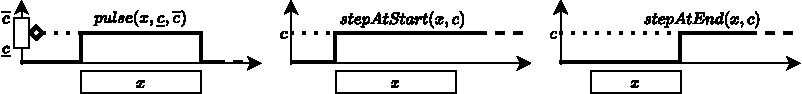
\includegraphics[width=\linewidth]{elementary.pdf}
    \caption{Elementary cumulative functions: \texttt{pulse}, \texttt{stepAtStart}, and \texttt{stepAtEnd}. Each function receives a conditional time-interval variable $x_i$ and a height $c_i$. (Figure from~\cite{Schaus2025GeneralizedCumulative}.)}
    \label{fig:elementary}
\end{figure}

Cumulative functions can be combined using the following operators as illustrated in Figure~\ref{fig:cumul-ast}:
\begin{itemize}
    \item \texttt{sum(f1, f2, ...)}: sum of multiple cumulative functions.
    \item \texttt{minus(f1, f2)}: difference of two functions.
\end{itemize}

The resulting cumulative function can be viewed as a cumulative expression or AST that can then be flattened to extract individual cumulative tasks
as illustrated in the left part of Figure~\ref{fig:cumul-ast} and explained in details in \cite{Schaus2025GeneralizedCumulative}.

\begin{figure}[t]
    \centering
    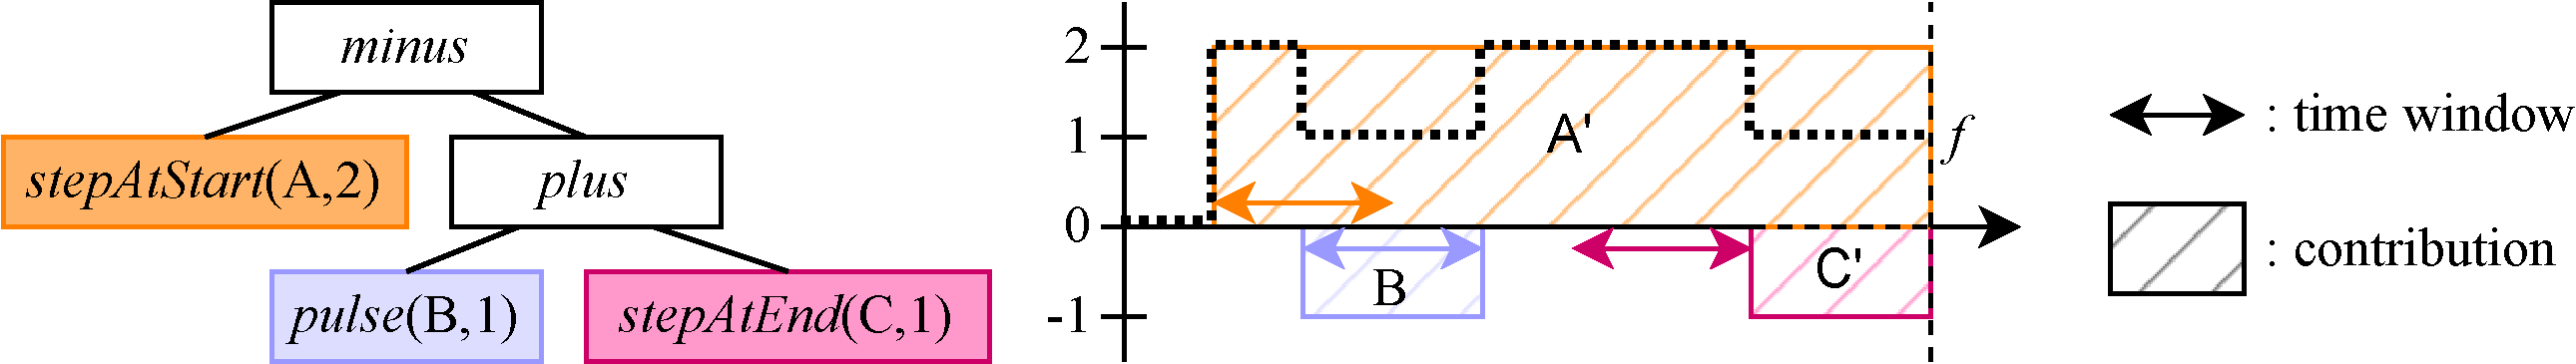
\includegraphics[width=\linewidth]{exampleCumul.pdf}
    \caption{Left: AST for the cumulative function $f = \textit{stepAtStart}(A, 2) - (\textit{pulse}(B, 1) + \textit{stepAtEnd}(C, 1))$. Right: the resulting cumulative function profile. Solid rectangles represent the time windows of the tasks; hatched areas show their contributions to the profile. (Figure from~\cite{Schaus2025GeneralizedCumulative}.)}
    \label{fig:cumul-ast}
\end{figure}


The height of a cumulative function can be bounded:
\begin{itemize}
    \item \texttt{le(f, maxCapa)}: the function $f$ must not exceed \texttt{maxCapa} at any time where at least one task executes.
    \item \texttt{alwaysIn(f, minCapa, maxCapa)}: the function $f$ must stay between \texttt{minCapa} and \texttt{maxCapa}.
\end{itemize}

Internally, these constraints are compiled into a single \gcumulative\ constraint~\cite{Schaus2025GeneralizedCumulative},
which accepts tasks with variable, possibly negative heights.
The task variables are extracted from the cumulative function expression by traversing its AST through a flattening process.

It is important to note that the \gcumulative\ constraint is more general than the classical cumulative constraint, which only allows positive heights and fixed tasks.
This constraint enforces the cumulative bounds at every time point where at least one task executes.
The formal semantics is given by the following definition.
\begin{definition}[\gcumulative]
The $\gcumulative(T, \minC, \maxC)$ constraint enforces that the cumulated heights of the tasks in $T$ lie within $[\minC, \maxC]$ at every time point at which at least one task executes:
\[
    \sum_{i \in R \mid s_i \leq \tau < e_i} c_i \in [\minC, \maxC] \qquad \forall \tau \in \bigcup_{i \in R} [s_i, e_i)
\]
where $R$ is the set of required (present) tasks and $c_i$ is the height of task $i$.
\end{definition}


\subsection{Modeling the RCPSP}

The Resource-Constrained Project Scheduling Problem (RCPSP) is a classical scheduling benchmark. Each activity has a fixed duration, consumes one or more resources, and must respect precedence constraints.
Unlike the Job-Shop where machines impose a \emph{no-overlap} requirement (unit capacity), the RCPSP involves \emph{cumulative} resources with capacity greater than one: multiple activities may execute simultaneously on the same resource, as long as their total consumption does not exceed the capacity.
This is modeled using cumulative function expressions. Listing~\ref{lst:rcpsp} shows the \maxicp\ model using the raw API.

\begin{codebox}[label={lst:rcpsp}]{RCPSP model (raw API)}
CPSolver cp = makeSolver();

CPIntervalVar[] tasks = makeIntervalVarArray(cp, nActivities);
for (int i = 0; i < nActivities; i++) {
    tasks[i].setLength(duration[i]);
    tasks[i].setPresent();
}

// Cumulative resources
CPCumulFunction[] resources = new CPCumulFunction[nResources];
for (int r = 0; r < nResources; r++) {
    resources[r] = new CPFlatCumulFunction();
}

for (int i = 0; i < nActivities; i++) {
    for (int r = 0; r < nResources; r++) {
        if (consumption[r][i] > 0) {
            resources[r] = new CPPlusCumulFunction(
                resources[r],
                new CPPulseCumulFunction(tasks[i], consumption[r][i])
            );
        }
    }
}

for (int r = 0; r < nResources; r++) {
    cp.post(le(resources[r], capa[r]));
}

// Precedences
for (int i = 0; i < nActivities; i++) {
    for (int k : successors[i]) {
        cp.post(endBeforeStart(tasks[i], tasks[k]));
    }
}

CPIntVar makespan = makespan(tasks);
Objective obj = cp.minimize(makespan);

DFSearch dfs = makeDfs(cp, fds(tasks));
dfs.optimize(obj);
\end{codebox}

The resource profile is built compositionally:
\texttt{CPFlatCumulFunction} represents the zero function, and for each activity consuming resource~$r$,
a \texttt{CPPulseCumulFunction} (contributing the consumption height while the task executes) is added using \texttt{CPPlusCumulFunction}.
The \texttt{le(resource, capa)} constraint ensures the cumulative profile never exceeds the capacity.
The search uses the Failure-Directed Search heuristic \texttt{fds}~\cite{failureDirectedSearch}.

\subsection{Producer-Consumer Scheduling}

Cumulative functions excel at modeling producer-consumer problems.
Consider a reservoir with limited capacity: producer tasks add to the level at their completion,
and consumer tasks remove from it at their start. Listing~\ref{lst:reservoir} shows this using the raw API.

\begin{codebox}[label={lst:reservoir}]{Producer-consumer with cumulative functions (raw API)}
CPCumulFunction reservoir = new CPFlatCumulFunction();

for (int i = 0; i < nProducers; i++) {
    reservoir = new CPPlusCumulFunction(
        reservoir,
        stepAtEnd(producerTask[i], producerQty[i])
    );
}

for (int i = 0; i < nConsumers; i++) {
    reservoir = new CPPlusCumulFunction(
        reservoir,
        stepAtStart(consumerTask[i], -consumerQty[i])
    );
}

cp.post(alwaysIn(reservoir, 0, capacity));
\end{codebox}

The \texttt{stepAtEnd(task, qty)} adds \texttt{qty} to the function at the task's end (the producer finishes and adds inventory).
The \texttt{stepAtStart(task, -qty)} subtracts at the task's start (the consumer begins and removes inventory).
The \texttt{alwaysIn} constraint ensures the reservoir level stays between 0 and the capacity at all times.



% ==================================================================================
\section{Sequence Variables for Routing}
\label{sec:seqvar}
% ==================================================================================

Vehicle Routing Problems (VRP) are among the most important applications of constraint programming. Traditional CP models for routing use \emph{successor arrays}, where an integer variable $\mathit{succ}_i$ represents the direct successor of node $i$ in the tour. While functional, this representation has significant limitations: it does not naturally support optional visits, and it cannot support insertion-based search heuristics, which are critical for quickly finding good solutions in practice.

\maxicp\ introduces \emph{sequence variables}~\cite{Schaus2022SeqVar}, a dedicated computational domain for routing and sequencing problems. Unlike the successor model, sequence variables represent a partial, growing path through node insertions, and natively support optional visits and insertion-based branching.

\subsection{Domain of a Sequence Variable}

A sequence variable $\seq{S}$ represents an ordered sequence of pairwise distinct nodes from a set $\nodes$, starting at an origin $\first$ and ending at a destination $\last$.
Its domain is represented intensionally as a tuple $\extDom = \langle R, X, \seq{s}, \NB \rangle$, where:

\begin{itemize}
    \item $R \subseteq \nodes$ is the set of \emph{required} nodes that must appear in every feasible sequence.
    \item $X \subseteq \nodes$ is the set of \emph{excluded} nodes that may not appear in any feasible sequence.
    \item $\seq{s}$ is a mandatory \emph{partial sequence}: a subsequence that must appear in every feasible sequence.
    \item $\NB \subseteq \nodes^3$ is a set of \emph{NotBetween} triples: for each $(i, j, k) \in \NB$, node $j$ is forbidden from appearing between $i$ and $k$.
\end{itemize}

\begin{definition}[Sequence Variable Domain]
The set of values represented by $\langle R, X, \seq{s}, \NB \rangle$ is:
\[
\llbracket \langle R, X, \seq{s}, \NB \rangle \rrbracket
=
\left\{
\seq{t} \in \mathcal{S}(\nodes)
\;\middle|\;
\begin{aligned}
& \text{$\seq{t}$ is a simple $(\first,\last)$-path}, \\
& R \subseteq \mathrm{nodes}(\seq{t}), \;
  \mathrm{nodes}(\seq{t}) \cap X = \varnothing, \\
& \seq{s} \preceq \seq{t}, \\
& \forall (i,j,k) \in \NB:\;
  \neg(i \prec j \prec k \text{ in } \seq{t})
\end{aligned}
\right\}
\]
\end{definition}

The four elementary domain restrictions are monotonic: adding elements to $R$, $X$, or $\NB$, or extending $\seq{s}$, yields a smaller (more constrained) domain. This provides a natural basis for incremental propagation.

Nodes are classified into four categories, illustrated in Figure~\ref{fig:seqvar_full}:

\begin{itemize}
    \item \textbf{Member}: nodes currently in the partial sequence $\seq{s}$.
    \item \textbf{Possible}: nodes that may or may not be in the final sequence (neither required nor excluded, and not yet inserted).
    \item \textbf{Required}: nodes that must be in the final sequence but are not yet inserted into $\seq{s}$.
    \item \textbf{Excluded}: nodes that have been removed from all feasible sequences.
\end{itemize}

\begin{figure}[t]
    \centering
    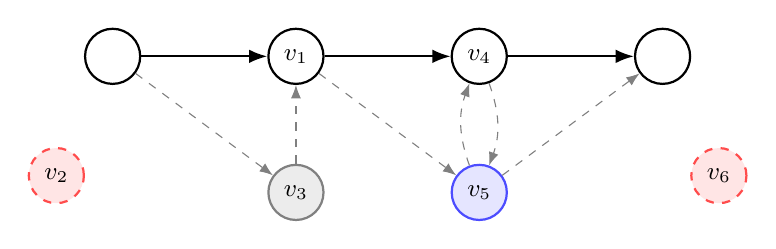
\begin{tikzpicture}[node distance=1.4cm and 1.6cm, >=LaTeX]
        % Members in the partial sequence
        \node [member](first) {$\first$};
        \node [member, right=of first] (v1) {$v_1$};
        \node [member, right=of v1] (v4) {$v_4$};
        \node [member, right=of v4] (last) {$\last$};

        % Other nodes
        \node [excluded, below left=1cm and 0.2cm of first] (v2) {$v_2$};
        \node [possible, below=1cm of v1] (v3) {$v_3$};
        \node [required, below=1cm of v4] (v5) {$v_5$};
        \node [excluded, below right=1cm and 0.2cm of last] (v6) {$v_6$};

        % Successor edges (the partial sequence)
        \draw [successor] (first) -- (v1);
        \draw [successor] (v1) -- (v4);
        \draw [successor] (v4) -- (last);

        % Insertion edges (dashed)
        \draw [insertionDirected] (first) edge[bend left=0] (v3);
        \draw [insertionDirected] (v3) edge[bend left=0] (v1);
        \draw [insertionDirected] (v1) edge[bend left=0] (v5);
        \draw [insertionDirected] (v5) edge[bend left=20] (v4);
        \draw [insertionDirected] (v4) edge[bend left=20] (v5);
        \draw [insertionDirected] (v5) edge[bend left=0] (last);
    \end{tikzpicture}
    \caption{Domain of a sequence variable. Solid arrows form the partial sequence $(\first, v_1, v_4, \last)$. Dashed arrows indicate feasible insertions. Node $v_3$ is possible (gray), $v_5$ is required (blue border), and $v_2, v_6$ are excluded (red, dashed border).}
    \label{fig:seqvar_full}
\end{figure}

\subsection{Compact Encoding}

The domain $\extDom$ is stored as a graph with $O(|\nodes|^2)$ memory.
The partial sequence $\seq{s}$ is maintained as a doubly-linked list.
For each node $v$ not in $\seq{s}$, the set of feasible insertion positions is represented as the set of member nodes after which $v$ can be inserted.
A pair $(u, v)$ means ``$v$ can be inserted immediately after $u$ in $\seq{s}$.'' The NotBetween triples $\NB$ are encoded by removing the corresponding insertion pair, under the restriction that the extremities of each NotBetween belong to $\seq{s}$.

Domain updates are:
\begin{itemize}
    \item \texttt{insert(pred, node)}: insert \texttt{node} after \texttt{pred} in $\seq{s}$.
    \item \texttt{exclude(node)}: remove \texttt{node} from all feasible sequences.
    \item \texttt{require(node)}: mark \texttt{node} as required.
    \item \texttt{removeInsert(pred, node)}: remove the insertion pair (\texttt{pred}, \texttt{node}).
\end{itemize}

All updates are reversible through the state management system.

\subsection{Global Constraints for Sequence Variables}

\maxicp\ provides several global constraints tailored for sequence variables:

\paragraph{\texttt{distance(SeqVar seqVar, int[][] dist, IntExpression totalDist)}.}
It links the total distance of the route to the total distance variable,
based on a distance matrix.

\paragraph{\texttt{transitionTimes(SeqVar seqVar, IntExpression[] time, int[][] dist)}.}
It enforces temporal consistency along the sequence \texttt{seqVar} using transition times between nodes.
Each node $v$ is associated with a variable $\textit{time}[v]$ representing the start time of its service (typically constrained by a time window).
For every pair of nodes $(u, v)$ such that $u$ precedes $v$ in \texttt{seqVar}, the constraint enforces:
$$
\textit{time}[u] + d_{u,v} \leq \textit{time}[v].
$$
This ensures that node $v$ cannot be started before reaching it from $u$.
The use of an inequality allows waiting at node $v$ (i.e., arriving earlier than its earliest start time).
Nodes that are not present in \texttt{seqVar} are not constrained.

\paragraph{\texttt{cumulative(SeqVar seqVar, int[] starts, int[] ends, int[] load, int capacity)}.}
It enforces capacity constraints for pickup-and-delivery activities along the sequence \texttt{seqVar}.
Introduced in \cite{thomas2020insertion}, it allows the modeling of the evolution of the vehicle load along the route:
picking up a request increases the load,
and delivering it decreases the load,
while ensuring feasibility at all times.

Each activity $i$ is defined by a pickup node $\textit{starts}[i]$,
a delivery node $\textit{ends}[i]$,
and a load $\textit{load}[i]$ that is carried from the pickup to the delivery.
The constraint ensures that:
\begin{itemize}
    \item Capacity constraint. At every node $v$ in \texttt{seqVar}, the total load of all active activities does not exceed the vehicle capacity:
$$
\sum_{i \mid \textit{starts}[i] \preceq v \prec \textit{ends}[i]} \textit{load}[i] \le \textit{capacity}.
$$
An activity contributes to the load between its pickup and its delivery.
\item Pairing of nodes. For each activity $i$, the pickup and delivery nodes are either both present in \texttt{seqVar} or both absent.
\item Precedence. If an activity is performed, its pickup node must appear before its delivery node in \texttt{seqVar}.
\end{itemize}

\subsection{Modeling the TSPTW}

The Traveling Salesman Problem with Time Windows (TSPTW)
is a classical routing problem.
In \maxicp, it can be modeled using either integer variables or
sequence variables.
We first show the integer-variable model (Listing~\ref{lst:tsptw}),
which uses a position-based formulation,
and then the sequence-variable model (Listing~\ref{lst:tsptw-seqvar}) used in \cite{delecluse2022sequence}.

\begin{codebox}[label={lst:tsptw}]{TSPTW with integer variables (raw API)}
CPSolver cp = makeSolver();

// x[i] is the node visited at position i
CPIntVar[] x = makeIntVarArray(cp, n, n);
// arrival[i] is the arrival time at position i
CPIntVar[] arrival = makeIntVarArray(cp, n, horizon);

cp.post(allDifferent(x));
cp.post(eq(x[0], 0));         // start at depot
cp.post(eq(x[n-1], n-1));     // end at depot copy
cp.post(eq(arrival[0], 0));   // depart at time 0

for (int i = 0; i < n; i++) {
    CPIntVar earliest = element(inst.earliest, x[i]);
    CPIntVar latest = element(inst.latest, x[i]);
    cp.post(le(earliest, arrival[i]));
    cp.post(le(arrival[i], latest));
}

CPIntVar[] transition = new CPIntVar[n - 1];
for (int i = 0; i < n - 1; i++) {
    transition[i] = element(distMatrix, x[i], x[i+1]);
    cp.post(le(sum(arrival[i], transition[i]),
               arrival[i+1]));
}

CPIntVar distance = sum(transition);
DFSearch search = makeDfs(cp, staticOrderBinary(x));
search.optimize(cp.minimize(distance));
\end{codebox}

Here, \texttt{element(T, x[i])} is the \emph{element} constraint that returns $T[x_i]$, enabling indexing into data arrays with decision variables. The two-dimensional variant \texttt{element(T, x[i], x[i+1])} retrieves $T[x_i][x_{i+1}]$.

The TSPTW can also be modeled with a sequence variable, which provides a more natural representation. Listing~\ref{lst:tsptw-seqvar} shows this model.

\begin{codebox}[label={lst:tsptw-seqvar}]{TSPTW with a sequence variable (raw API)}
CPSolver cp = makeSolver();

CPSeqVar tour = makeSeqVar(cp, n, 0, n - 1);
for (int i = 0; i < n; i++)
    tour.require(i);  // all nodes must be visited

CPIntVar[] time = makeIntVarArray(cp, n, horizon);
cp.post(eq(time[0], 0));
for (int i = 1; i < n; i++) {
    time[i].removeAbove(latest[i]);
    time[i].removeBelow(earliest[i]);
}

cp.post(new TransitionTimes(tour, time, distMatrix));

CPIntVar totDist = makeIntVar(cp, 0, 100000);
cp.post(new Distance(tour, distMatrix, totDist));

DFSearch dfs = makeDfs(cp, /* insertion search */);

dfs.optimize(cp.minimize(totDist));
\end{codebox}

The \texttt{CPSeqVar} represents a path from node 0 (depot) to node $n{-}1$ (depot copy). Each node is required using \texttt{tour.require(i)}. The \texttt{TransitionTimes} constraint links the time-window variables and enforces travel times between consecutive nodes. The \texttt{Distance} constraint bounds the total distance.

\subsection{Custom Insertion-Based Search}

Built-in heuristics such as \texttt{firstFailBinary(seqVars)} (Section~\ref{sec:search}) are convenient, but routing problems often benefit from a custom insertion-based search. Writing one requires querying the sequence variable's domain at each search node. The key API methods are:

\begin{itemize}
    \item \texttt{tour.isFixed()}: returns \texttt{true} when all nodes are either members or excluded.
    \item \texttt{tour.fillNode(nodes, INSERTABLE)}: fills the array with nodes that are not yet in the partial sequence and returns their count.
    \item \texttt{tour.nInsert(node)}: returns the number of feasible insertion points for a node.
    \item \texttt{tour.fillInsert(node, preds)}: fills the array with the member nodes after which \texttt{node} can be inserted, and returns their count.
    \item \texttt{tour.memberAfter(pred)}: returns the current successor of \texttt{pred} in the partial sequence.
\end{itemize}

Listing~\ref{lst:custom-search-seqvar} shows a custom branching for the TSP. At each search node, the heuristic (i)~selects the insertable node with the fewest insertion points (first-fail on insertions), (ii)~among its feasible insertion positions, picks the one with the smallest \emph{detour cost} $d_{\mathit{pred},\mathit{node}} + d_{\mathit{node},\mathit{succ}} - d_{\mathit{pred},\mathit{succ}}$, and (iii)~creates a binary branching: insert the node at that position on the left, or forbid that placement with a \texttt{notBetween} constraint on the right.

\begin{codebox}[label={lst:custom-search-seqvar}]{Custom insertion-based search for the TSP (raw API)}
int[] nodes = new int[n];
DFSearch dfs = makeDfs(cp, () -> {
    if (tour.isFixed()) return EMPTY;

    // Variable selection: node with fewest insertion points
    int nInsertable = tour.fillNode(nodes, INSERTABLE);
    int node = selectMin(nodes, nInsertable,
        i -> true, tour::nInsert).getAsInt();

    // Value selection: insertion with smallest detour
    int nInsert = tour.fillInsert(node, nodes);
    int bestPred = selectMin(nodes, nInsert,
        pred -> true,
        pred -> {
            int succ = tour.memberAfter(pred);
            return dist[pred][node] + dist[node][succ]
                 - dist[pred][succ];
        }).getAsInt();
    int succ = tour.memberAfter(bestPred);

    // Binary branch: insert or forbid this placement
    return branch(
        () -> cp.post(insert(tour, bestPred, node)),
        () -> cp.post(notBetween(tour, bestPred, node, succ))
    );
});
\end{codebox}

The \texttt{insert(tour, pred, node)} constraint inserts \texttt{node} immediately after \texttt{pred} in the partial sequence, so that the path becomes $\ldots \to \mathit{pred} \to \mathit{node} \to \mathit{succ} \to \ldots$\,.
The \texttt{notBetween(tour, pred, node, succ)} constraint forbids \texttt{node} from appearing between \texttt{pred} and \texttt{succ} in any feasible sequence, effectively pruning that insertion point without committing to a specific alternative.
This binary branching mirrors the assign/remove pattern of \texttt{heuristicBinary} for integer variables: the left branch commits to the best insertion, while the right branch eliminates it and lets the search explore other placements.

\subsection{Vehicle Routing with Sequence Variables}

For multi-vehicle routing, sequence variables truly shine. Listing~\ref{lst:vrptw} shows a Capacitated Vehicle Routing Problem with Time Windows (CVRPTW) model using the raw API, based on the Solomon benchmarks.

\begin{codebox}[label={lst:vrptw}]{CVRPTW with sequence variables (raw API)}
CPSolver cp = makeSolver();
CPSeqVar[] vehicles = new CPSeqVar[nVehicle];
CPIntVar[] time = new CPIntVar[nNode];
CPIntVar[] distance = new CPIntVar[nVehicle];

for (int v = 0; v < nVehicle; v++) {
    vehicles[v] = makeSeqVar(cp, nNode,
        nRequest + v * 2, nRequest + v * 2 + 1);
    distance[v] = makeIntVar(cp, 0, depotEnd);
}
for (int i = 0; i < nRequest; i++)
    time[i] = makeIntVar(cp, twStart[i], twEnd[i]);
for (int i = nRequest; i < nNode; i++)
    time[i] = makeIntVar(cp, depotStart, depotEnd);

for (int v = 0; v < nVehicle; v++) {
    cp.post(new TransitionTimes(
        vehicles[v], time, distMatrix, duration));
    // Capacity + pickup-before-delivery + same vehicle
    cp.post(new Cumulative(
        vehicles[v], pickups, drops, load, capacity));
    cp.post(new Distance(
        vehicles[v], distMatrix, distance[v]));
}
CPIntVar sumDist = sum(distance);

// Each node visited exactly once across all vehicles
for (int node = 0; node < nNode; node++) {
    CPIntVar[] visits = new CPIntVar[nVehicle];
    for (int v = 0; v < nVehicle; v++)
        visits[v] = vehicles[v].getNodeVar(node)
                                .isRequired();
    cp.post(new Sum(visits, 1));
}

DFSearch search = makeDfs(cp, /* insertion search */);
search.optimize(cp.minimize(sumDist));
\end{codebox}

Each vehicle is represented by a \texttt{CPSeqVar} with its own start and end depot nodes. The \texttt{getNodeVar(node).isRequired()} method returns a 0/1 \texttt{CPIntVar} indicating whether the node is required (assigned) to that vehicle. The capacity is enforced by summing the loads of the required nodes.  The constraint $\sum_v \texttt{visits}_v = 1$ ensures each customer is served by exactly one vehicle.

\subsection{Pickup and Delivery with Sequence Variables}

The Dial-A-Ride Problem (DARP) is a Pickup and Delivery Problem with time windows, load capacity, and ride-time constraints. Each request has a pickup node and a delivery node; the vehicle must visit the pickup before the delivery while respecting its capacity. Listing~\ref{lst:pdp} shows the model using the raw API.

\begin{codebox}[label={lst:pdp}]{DARP with sequence variables and cumulative load (raw API)}
CPSolver cp = makeSolver();
CPSeqVar[] routes = new CPSeqVar[nVehicle];
CPIntVar[] time = new CPIntVar[n];
CPIntVar[] distance = new CPIntVar[nVehicle];

for (int v = 0; v < nVehicle; v++) {
    routes[v] = makeSeqVar(cp, n,
        rangeDepot + v, rangeDepot + nVehicle + v);
    distance[v] = makeIntVar(cp, 0, maxDist);
}
for (int i = 0; i < n; i++)
    time[i] = makeIntVar(cp, twStart[i], twEnd[i]);

int[] pickups = IntStream.range(0, nRequest).toArray();
int[] drops = IntStream.range(nRequest, 2*nRequest).toArray();

for (int v = 0; v < nVehicle; v++) {
    cp.post(new TransitionTimes(
        routes[v], time, distMatrix, duration));
    // Capacity + pickup-before-delivery + same vehicle
    cp.post(new Cumulative(
        routes[v], pickups, drops, load, capacity));
    cp.post(new Distance(
        routes[v], distMatrix, distance[v]));
}

// Max ride time: time[drop] <= time[pickup] + dur + maxRide
for (int i = 0; i < nRequest; i++)
    cp.post(new LessOrEqual(time[i + nRequest],
        plus(time[i], duration[i] + maxRideTime)));

// Each node visited exactly once
for (int node = 0; node < n; node++) {
    CPIntVar[] visits = new CPIntVar[nVehicle];
    for (int v = 0; v < nVehicle; v++)
        visits[v] = routes[v].getNodeVar(node).isRequired();
    cp.post(new Sum(visits, 1));
}

CPIntVar sumDist = sum(distance);
DFSearch search = makeDfs(cp, /* insertion search */);
search.optimize(cp.minimize(sumDist));
\end{codebox}

The \texttt{Cumulative} constraint on a sequence variable is particularly powerful: it simultaneously enforces the vehicle capacity, ensures each request's pickup precedes its delivery, and guarantees that both nodes of a request are assigned to the same vehicle. The \texttt{LessOrEqual} constraint enforces the maximum ride time for each request.

\subsection{LNS with Sequence Variables}
\label{sec:lns-seqvar}

Sequence variables are ideally suited for Large Neighborhood Search. A destroy-and-repair cycle consists of:
\begin{enumerate}
    \item \textbf{Destroy}: select a set of nodes to relax.
    \item \textbf{Repair}: enforce the previous solution except for relaxed nodes, then search for new insertions.
\end{enumerate}

The key primitive is \texttt{RelaxedSequence}: given the current best tour stored in an array \texttt{bestTour} and a set of relaxed nodes, it constrains the sequence variable to follow the previous ordering for all non-relaxed nodes, while leaving the relaxed nodes free for re-insertion. 
Listing~\ref{lst:lns-seqvar} shows the LNS loop using the raw API.

\begin{codebox}[label={lst:lns-seqvar}]{LNS with sequence variables (raw API)}
int[] bestTour = IntStream.range(0, n + 1).toArray();

dfs.onSolution(() -> {
    tour.fillNode(bestTour, SeqStatus.MEMBER_ORDERED);
});

Random random = new Random(42);
for (int iter = 0; iter < 100; iter++) {
    dfs.optimizeSubjectTo(obj, s -> false, () -> {
        Set<Integer> relaxed = randomSubset(random, 0, n, 5);
        cp.post(new RelaxedSequence(tour, bestTour, relaxed));
    });
}
\end{codebox}

At each iteration, \texttt{optimizeSubjectTo} saves the solver state, posts the \texttt{RelaxedSequence} constraint that fixes all non-relaxed nodes in their best-known order, searches for improving solutions, and then restores the state. 
This follows the same pattern as the QAP LNS loop (Section~\ref{sec:lns}), but the \texttt{RelaxedSequence} constraint is specifically designed for sequence variables.


% ==================================================================================
\section{Symbolic Modeling with \maxicp-Modelling}
\label{sec:symbolism}
% ==================================================================================

Having covered the raw implementation layer---state management, propagation, search, sequence variables, scheduling, and multi-objective support---we now turn to the symbolic modeling layer.
As introduced in Section~\ref{sec:two-layer-overview}, \maxicp\ provides a higher-level API that separates the \emph{definition} of a model from its \emph{resolution}.
This is achieved through a symbolic modeling layer called \maxicp-Modelling~\cite{Derval2023Symbolism}, which treats models as first-class, immutable data structures.

\subsection{Models as Functional Linked Lists}

In \maxicp-Modelling, a \texttt{SymbolicModel} is an immutable record consisting of a constraint, a pointer to a parent model, and a reference to the \texttt{ModelProxy}. Adding a constraint to a model returns a \emph{new} model node, leaving the original unchanged:

\begin{codebox}{The SymbolicModel record}
public record SymbolicModel(
    Constraint constraint,
    SymbolicModel parent,
    ModelProxy modelProxy
) implements Model, Iterable<Constraint> {
    public SymbolicModel add(Constraint c) {
        return new SymbolicModel(c, this, modelProxy);
    }
}
\end{codebox}

Because models are immutable linked lists, adding a constraint is an $O(1)$ operation. The complete list of constraints can be recovered by traversing the chain to the root. This design enables the creation of \emph{model trees}, where each branch represents a different sub-problem, reformulation, or neighborhood.

\subsection{The \texttt{ModelDispatcher}}

The \texttt{ModelDispatcher} is the primary user-facing class for the symbolic layer. It maintains a thread-local reference to the current model and acts as both a variable factory and a model proxy. When the user calls \texttt{model.add(constraint)}, the dispatcher appends the constraint to the current symbolic model:

\begin{codebox}{Creating a model with the ModelDispatcher}
ModelDispatcher model = Factory.makeModelDispatcher();
IntVar[] x = model.intVarArray(n, n);
model.add(allDifferent(x));
model.add(eq(x[0], 0));
\end{codebox}

Variables are symbolic objects that do not belong to any concrete solver until concretization. This allows the same variables to be shared across multiple concrete solver instances.

\subsection{Concretization}

To solve a model, it must be \emph{concretized} into a solver engine. The \texttt{runCP} method on \texttt{ModelDispatcher} handles this:

\begin{codebox}{Concretizing and solving a model}
model.runCP(cp -> {
    DFSearch search = cp.dfSearch(firstFailBinary(x));
    SearchStatistics stats = search.solve();
});
\end{codebox}

Internally, this creates a \texttt{ConcreteCPModel} that:
\begin{enumerate}
    \item Creates a fresh \texttt{MaxiCP} solver instance with a \texttt{Trailer}.
    \item Iterates over the symbolic constraint list and \emph{instantiates} each one in the underlying CP engine. Symbolic expressions (e.g., \texttt{Sum}, \texttt{Element1D}) are translated into concrete CP variables and constraints through pattern matching in the \texttt{ConcreteCPModel} class.
    \item Runs the initial fixed-point propagation.
\end{enumerate}

The mapping between symbolic and concrete variables is maintained in reversible state maps, enabling incremental constraint addition during search.

\subsection{Model Transformations and Reformulations}

Because models are immutable trees, they support powerful compositional operations:

\paragraph{Neighborhoods for LNS.} A neighborhood is simply a model extension. Given a base model and a solution, one creates a new model by adding fixing constraints:

\begin{codebox}{LNS with symbolic models}
Model relaxed = base;
for (IntVar x : variables) {
    if (rand.nextDouble() > 0.1)
        relaxed = relaxed.add(eq(x, solution.get(x)));
}
relaxed.runCP(cp -> ...); // solve the neighborhood
\end{codebox}

Each neighborhood is a different branch of the model tree. The base model is never modified.
This approach to LNS complements the raw-level \texttt{optimizeSubjectTo} technique presented in Section~\ref{sec:lns}: while the raw API relies on save/restore of the solver state, the symbolic approach creates entirely independent model branches that can be solved concurrently.

\paragraph{Hybridization.} Although not implemented in \maxicp\ the same symbolic model could be transformed into input for a MIP solver (through linearization of supported constraints)
or solved concurrently by both a CP and a MIP engine.
We refer to \cite{van2013objective} for a detailed case study of CP/MIP hybridization using symbolic modeling.

\subsection{Embarrassingly Parallel Search}
\label{sec:eps}

Embarrassingly Parallel Search (EPS)~\cite{regin2013embarrassingly,malapert2016embarrassingly} is a simple yet effective approach to parallelizing constraint solving.
The idea is to decompose the original problem into a large number of independent sub-problems that can be solved concurrently with no communication between workers.
Concretely, the search tree is explored up to a fixed depth~$d$ using the normal branching heuristic.
Each leaf of this depth-limited exploration defines a sub-problem: the original model augmented with the branching decisions made along the path from the root to that leaf.
These sub-problems are then dispatched to a thread pool for independent resolution.
Because the sub-problems are disjoint (they partition the search space), the total solution count---or the global optimum---can be computed by simply aggregating the individual results.

The symbolic modeling layer of \maxicp\ makes EPS particularly natural to implement.
Since models are immutable linked lists, the branching decisions applied during the decomposition phase produce new symbolic model nodes without modifying the original model.
At each leaf of the depth-limited search, a call to \texttt{cp.symbolicCopy()} captures the current sub-problem as a standalone symbolic model.
This model can then be concretized and solved in a separate thread, with no shared mutable state.

Listing~\ref{lst:nqueens-eps} illustrates EPS on the N-Queens problem.
The model and branching heuristic are identical to those shown in Listing~\ref{lst:nqueens-modeling}.
The decomposition wraps the branching in a \texttt{LimitedDepthBranching} combinator that stops at depth~10, causing the search to treat each leaf as a ``solution.''
For each such leaf, \texttt{cp.symbolicCopy()} extracts the corresponding sub-problem, which is submitted to a fixed thread pool of 8 workers.
Each worker concretizes the sub-problem into a fresh solver instance and runs a complete search.
Finally, the solution counts are summed.

\begin{codebox}[label={lst:nqueens-eps}]{N-Queens solved with EPS}
// model and branching defined as in Listing 2
ExecutorService executor = Executors.newFixedThreadPool(8);

Function<Model, SearchStatistics> epsSolve = (m) -> {
    return model.runAsConcrete(
        CPModelInstantiator.withTrailing, m, (cp) -> {
        DFSearch search = cp.dfSearch(branching);
        return search.solve();
    });
};

LinkedList<Future<SearchStatistics>> results = new LinkedList<>();
model.runCP((cp) -> {
    DFSearch search = cp.dfSearch(
        new LimitedDepthBranching(branching, 10));
    search.onSolution(() -> {
        Model m = cp.symbolicCopy(); // capture sub-problem
        results.add(executor.submit(
            () -> epsSolve.apply(m)));
    });
    search.solve(); // decompose
});

int total = 0;
for (var f : results)
    total += f.get().numberOfSolutions();
System.out.println("Total solutions: " + total);
executor.shutdown();
\end{codebox}

The key enabler is that \texttt{symbolicCopy()} returns a lightweight, immutable snapshot of the model at the current search node.
Because each sub-problem is concretized independently, there is no shared solver state and therefore no synchronization overhead.
The depth parameter~$d$ controls the granularity of the decomposition: a larger~$d$ produces more and smaller sub-problems, which improves load balancing at the cost of a longer decomposition phase.

Since symbolic models are immutable and variables are symbolic, the same model can also be safely shared across multiple threads for portfolio-style parallel search. Each thread independently concretizes the model and explores the search space with a different heuristic or random seed:

\begin{codebox}{Portfolio parallel search with symbolic models}
ModelDispatcher model = ...; // build the model
IntStream.range(0, nThreads).parallel().forEach(t -> {
    model.runCP(cp -> {
        DFSearch search = cp.dfSearch(
            randomizedFirstFail(x, new Random(t)));
        search.optimize(minimize(cost));
    });
});
\end{codebox}


\subsection{Mixing Both Layers}

Inside the \texttt{runCP} callback, the user has access to both the concrete model and the symbolic variables. The concrete model allows accessing the underlying \texttt{CPVar} objects, which is useful for implementing custom search heuristics that need direct access to domain internals.


% ==================================================================================
\section{Conclusion}
\label{sec:conclusion}
% ==================================================================================

We have presented \maxicp, a modern,
open-source constraint programming solver that bridges the gap
between educational simplicity and industrial-grade performance.
By building on the architectural clarity of \minicp\ and incorporating ideas from \oscar\ and \objectivecp,
\maxicp\ introduces three key functionalities that set it apart for an open-source CP solver:

\begin{enumerate}
    \item \textbf{Conditional time intervals and cumulative functions}: Full support for optional tasks, alternative resources, and producer-consumer scheduling through the Generalized Cumulative constraint.
    \item \textbf{Sequence variables}: A dedicated computational domain for routing that supports optional visits, insertion-based heuristics, and LNS, with global constraints for distance, transition times, and cumulative load.
    \item \textbf{Symbolic modeling}: Models as immutable functional linked lists enable model transformations, LNS neighborhoods, hybridization with MIP solvers, and embarrassingly parallel search.
\end{enumerate}

The two-layer API design (raw and symbolic) makes \maxicp\ accessible to both beginners learning CP and
experts deploying it in production. The entire codebase is available as open-source under the MIT license.

Future work includes expanding the reformulation library (e.g., automatic linearization for MIP hybridization),
integrating advanced black-box heuristics,
and developing a MiniZinc backend.

\bibliographystyle{unsrtnat}
\bibliography{maxicp}

\end{document}
